\documentclass[border=14pt]{standalone}
\usepackage{tikz}
\usepackage{xcolor}
\usetikzlibrary{arrows.meta, decorations.markings}

%=========================== CONFIGURATION ===========================
\def\W{8}          % horizontal separation of the two space points (= \ell)
\def\Rise{4.5}     % vertical rise per one-way crossing (= \ell/v ; sets slope 1/v)
\def\Ncross{5}     % number of one-way crossings spanned by window (sets height)
\def\N{5}          % number of bins (sub-beams) tiling each group
\def\Span{90}      % total beam phase-width, in degrees, within (0,180)
\def\AwLen{5pt}    % arrowhead length
\def\AwPos{0.3}    % arrow position along each segment (off-centre to clear crossings)
\def\LeftOp{0.5}   % fill opacity of the up-going (reflected) bins
\def\Gap{2.6}      % vertical gap (in display) between the two stacked plots
\def\Ms{30}        % samples per half-period for the sinusoidal plot
%=====================================================================

% group 0 palette (cool) -- light enough for dark ink details on top
\definecolor{cA}{RGB}{78,121,167}   % steel blue
\definecolor{cB}{RGB}{118,183,178}  % teal
\definecolor{cC}{RGB}{89,161,79}    % green
% group 1 palette (warm) -- the 180-degree out-of-phase family
\definecolor{dA}{RGB}{124,81,140}   % muted purple
\definecolor{dB}{RGB}{201,99,104}   % muted coral
\definecolor{dC}{RGB}{232,168,90}   % warm amber
\definecolor{ink}{RGB}{27,30,43}

\begin{document}
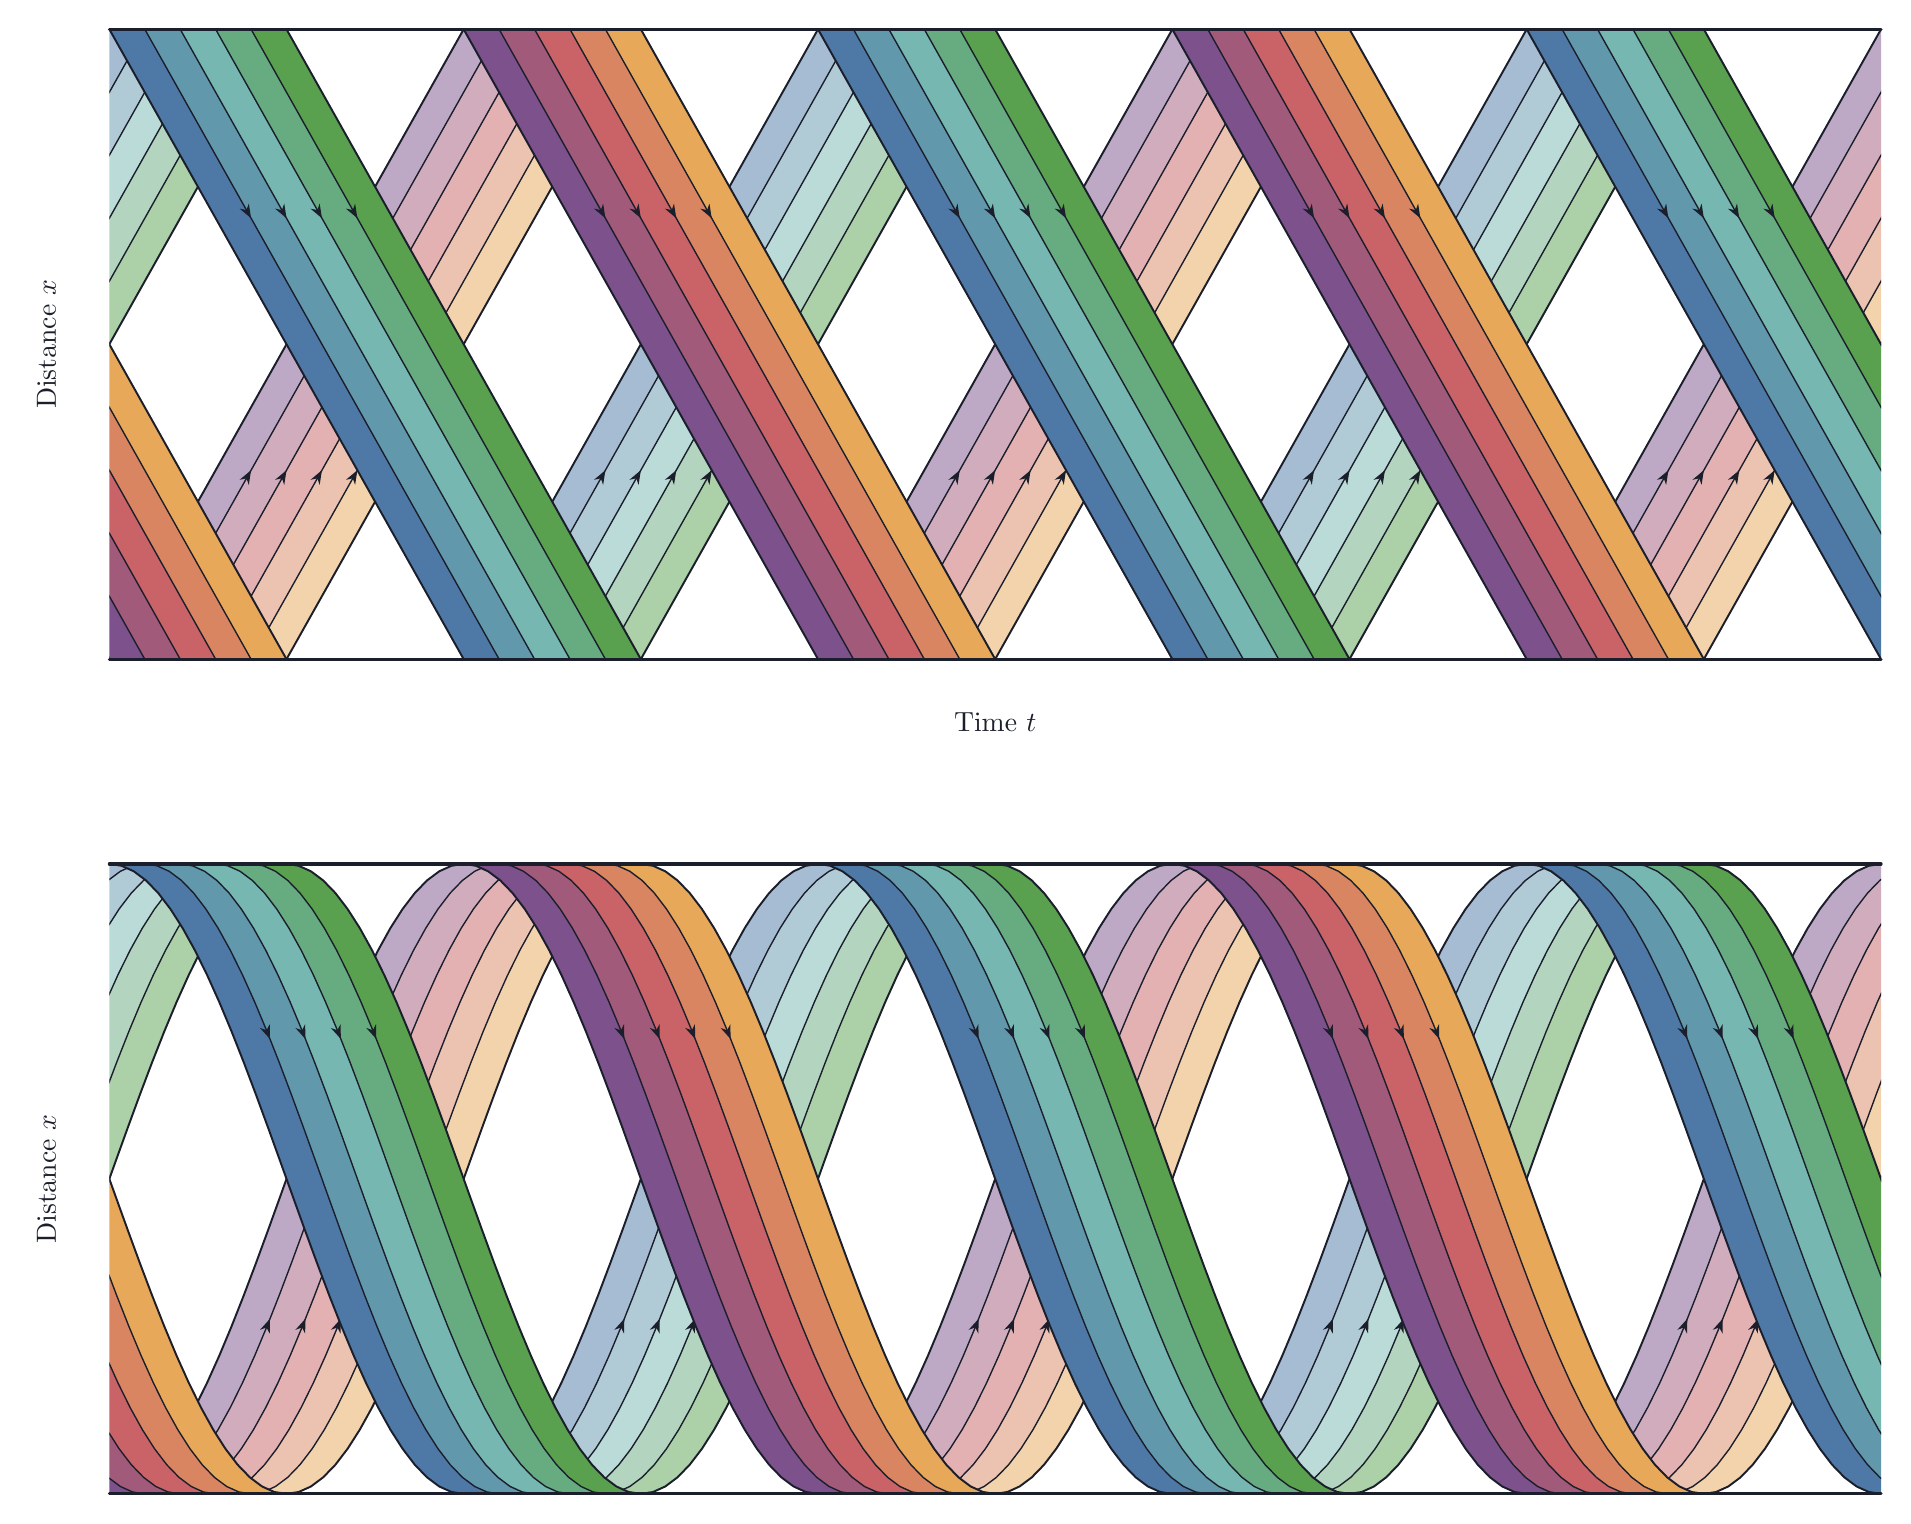
\begin{tikzpicture}[rotate=-90, line cap=round, line join=round]
  \pgfmathsetmacro{\H}{\Ncross*\Rise}
  \pgfmathsetmacro{\Beam}{\Span/180*\Rise}     % total beam time-width
  \pgfmathsetmacro{\binw}{\Beam/\N}            % per-bin time-width
  \pgfmathtruncatemacro{\imin}{-2}
  \pgfmathtruncatemacro{\imax}{\Ncross}
  \pgfmathtruncatemacro{\Nm}{\N-1}

  \begin{scope}
    \clip (0,0) rectangle (\W,\H);

    % Outer loop on direction so the rule is global: every up-going (reflected)
    % element of BOTH phase groups is drawn first and at \LeftOp opacity; every
    % down-going (forward) element is drawn afterwards, opaque, on top.
    % Inner loop on \g adds the second group: \g=1 is shifted +\Rise (=180 deg,
    % the opposite phase) and uses the warm palette.
    \foreach \dir in {1,0}{
      \ifnum\dir=1 \def\fillop{\LeftOp}\else \def\fillop{1}\fi
      \foreach \g in {0,1}{
        \pgfmathsetmacro{\goff}{\g*\Rise}
        \ifnum\g=0
          \colorlet{kA}{cA}\colorlet{kB}{cB}\colorlet{kC}{cC}
        \else
          \colorlet{kA}{dA}\colorlet{kB}{dB}\colorlet{kC}{dC}
        \fi

        % ---- filled bins ----
        \foreach \k in {0,...,\Nm}{
          \pgfmathsetmacro{\f}{\N==1 ? 0 : \k/(\N-1)}
          \ifdim\f pt<0.5pt
            \pgfmathsetmacro{\p}{\f*200}\colorlet{binc}{kB!\p!kA}
          \else
            \pgfmathsetmacro{\p}{(\f-0.5)*200}\colorlet{binc}{kC!\p!kB}
          \fi
          \pgfmathsetmacro{\sa}{\k*\binw}
          \pgfmathsetmacro{\sb}{(\k+1)*\binw}
          \foreach \i in {\imin,...,\imax}{
            \pgfmathtruncatemacro{\prt}{abs(mod(\i,2))}
            \ifnum\prt=\dir
              \pgfmathsetmacro{\xa}{\prt*\W}\pgfmathsetmacro{\xb}{(1-\prt)*\W}
              \pgfmathsetmacro{\ya}{\i*\Rise+\goff}\pgfmathsetmacro{\yb}{(\i+1)*\Rise+\goff}
              \fill[binc,fill opacity=\fillop] (\xa,\ya+\sa) -- (\xb,\yb+\sa) -- (\xb,\yb+\sb) -- (\xa,\ya+\sb) -- cycle;
            \fi
          }
        }

        % ---- internal dividers (where bins touch) with direction arrows ----
        \foreach \j in {1,...,\Nm}{
          \pgfmathsetmacro{\s}{\j*\binw}
          \foreach \i in {\imin,...,\imax}{
            \pgfmathtruncatemacro{\prt}{abs(mod(\i,2))}
            \ifnum\prt=\dir
              \pgfmathsetmacro{\xa}{\prt*\W}\pgfmathsetmacro{\xb}{(1-\prt)*\W}
              \pgfmathsetmacro{\ya}{\i*\Rise+\s+\goff}\pgfmathsetmacro{\yb}{(\i+1)*\Rise+\s+\goff}
              \draw[ink, line width=0.5pt,
                postaction={decorate, decoration={markings,
                  mark=at position \AwPos with {\arrow{Stealth[length=\AwLen]}}}}]
                (\xa,\ya) -- (\xb,\yb);
            \fi
          }
        }

        % ---- outer beam edges (outline only) ----
        \foreach \s in {0,\Beam}{
          \foreach \i in {\imin,...,\imax}{
            \pgfmathtruncatemacro{\prt}{abs(mod(\i,2))}
            \ifnum\prt=\dir
              \pgfmathsetmacro{\xa}{\prt*\W}\pgfmathsetmacro{\xb}{(1-\prt)*\W}
              \pgfmathsetmacro{\ya}{\i*\Rise+\s+\goff}\pgfmathsetmacro{\yb}{(\i+1)*\Rise+\s+\goff}
              \draw[ink, line width=0.7pt] (\xa,\ya) -- (\xb,\yb);
            \fi
          }
        }

      }
    }
  \end{scope}

  % ---- walls + centred axis titles ----
  \draw[ink, line width=1.15pt] (0,0) -- (0,\H);
  \draw[ink, line width=1.15pt] (\W,0) -- (\W,\H);
  \node[ink] at (\W+0.8,\H/2) {Time $t$};
  \node[ink,rotate=90] at (\W/2,-0.8) {Distance $x$};

  % =====================================================================
  %  SECOND PLOT (sinusoidal): a duplicate of the diagram above, shifted
  %  down by \Xoff in x, with each straight half-segment replaced by a
  %  half-cosine. The cosine extrema (troughs on xmin, peaks on xmax) land
  %  at exactly the same points/times as the straight reflection vertices.
  %  All other rules are identical: 5-bin gradient per group, the warm
  %  180-degree group, off-centre arrows, and the global down-on-top /
  %  opaque vs up-going / transparent ordering.
  % =====================================================================
  \pgfmathsetmacro{\Xoff}{\W+\Gap}
  \begin{scope}
    \clip (\Xoff,0) rectangle (\Xoff+\W,\H);
    \foreach \dir in {1,0}{
      \ifnum\dir=1 \def\fillop{\LeftOp}\else \def\fillop{1}\fi
      \foreach \g in {0,1}{
        \pgfmathsetmacro{\goff}{\g*\Rise}
        \ifnum\g=0
          \colorlet{kA}{cA}\colorlet{kB}{cB}\colorlet{kC}{cC}
        \else
          \colorlet{kA}{dA}\colorlet{kB}{dB}\colorlet{kC}{dC}
        \fi

        % ---- filled bins (sinusoidal bands) ----
        \foreach \k in {0,...,\Nm}{
          \pgfmathsetmacro{\f}{\N==1 ? 0 : \k/(\N-1)}
          \ifdim\f pt<0.5pt
            \pgfmathsetmacro{\p}{\f*200}\colorlet{binc}{kB!\p!kA}
          \else
            \pgfmathsetmacro{\p}{(\f-0.5)*200}\colorlet{binc}{kC!\p!kB}
          \fi
          \pgfmathsetmacro{\sa}{\k*\binw}
          \pgfmathsetmacro{\sb}{(\k+1)*\binw}
          \foreach \i in {\imin,...,\imax}{
            \pgfmathtruncatemacro{\prt}{abs(mod(\i,2))}
            \ifnum\prt=\dir
              \pgfmathsetmacro{\da}{\i*180}\pgfmathsetmacro{\db}{(\i+1)*180}
              \fill[binc,fill opacity=\fillop]
                plot[domain=\da:\db,samples=\Ms,variable=\t]
                  ({\Xoff+\W/2*(1-cos(\t))},{\sa+\goff+\Rise*\t/180})
                -- plot[domain=\db:\da,samples=\Ms,variable=\t]
                  ({\Xoff+\W/2*(1-cos(\t))},{\sb+\goff+\Rise*\t/180})
                -- cycle;
            \fi
          }
        }

        % ---- internal dividers (sinusoidal) with direction arrows ----
        \foreach \j in {1,...,\Nm}{
          \pgfmathsetmacro{\s}{\j*\binw}
          \foreach \i in {\imin,...,\imax}{
            \pgfmathtruncatemacro{\prt}{abs(mod(\i,2))}
            \ifnum\prt=\dir
              \pgfmathsetmacro{\da}{\i*180}\pgfmathsetmacro{\db}{(\i+1)*180}
              \draw[ink, line width=0.5pt,
                postaction={decorate, decoration={markings,
                  mark=at position \AwPos with {\arrow{Stealth[length=\AwLen]}}}}]
                plot[domain=\da:\db,samples=\Ms,variable=\t]
                  ({\Xoff+\W/2*(1-cos(\t))},{\s+\goff+\Rise*\t/180});
            \fi
          }
        }

        % ---- outer beam edges (sinusoidal) ----
        \foreach \s in {0,\Beam}{
          \foreach \i in {\imin,...,\imax}{
            \pgfmathtruncatemacro{\prt}{abs(mod(\i,2))}
            \ifnum\prt=\dir
              \pgfmathsetmacro{\da}{\i*180}\pgfmathsetmacro{\db}{(\i+1)*180}
              \draw[ink, line width=0.7pt]
                plot[domain=\da:\db,samples=\Ms,variable=\t]
                  ({\Xoff+\W/2*(1-cos(\t))},{\s+\goff+\Rise*\t/180});
            \fi
          }
        }

      }
    }
  \end{scope}

  % ---- walls + distance title for the second plot ----
  \draw[ink, line width=1.15pt] (\Xoff,0) -- (\Xoff,\H);
  \draw[ink, line width=1.15pt] (\Xoff+\W,0) -- (\Xoff+\W,\H);
  \node[ink,rotate=90] at (\Xoff+\W/2,-0.8) {Distance $x$};
\end{tikzpicture}
\end{document}
